\documentclass[9pt]{article}

\usepackage{algorithm}
\usepackage{algpseudocode}
\usepackage{caption}
\usepackage{amssymb}
\usepackage{graphicx}

\title{SSA Experiments on SMALLPRESENT-[$8$]}
\author{Md. Mohsin Ali Khan\\}

\begin{document}
\maketitle
\section{SSA Capacities}

\begin{center}
\begin{scriptsize}
\captionof{table}{SSA Capacities}
\begin{tabular}{l*{4}{c}r} \label{table:comparing_hypothesis}
Round & $C=$ & $\sigma^2_{C(a)}$ &  $\sigma^2_{C(a)}$ & Distance & Variance of $\sigma^2_{p_{\eta}(a)}$ \\
& $\frac{1}{2^8}\sum_{a \in \mathbb{F}_2^8}C(a)$ & (Experimental) & (Theoretical) & & (over all $\eta$)\\
\hline
1 & 1.25000000 & 0.5781250000000 & 0.01225490196078 & 0.56587009803921 & 0.000000000000000000000000\\
2 & 0.27648926 & 0.0145425647497 & 0.00059957889949 & 0.01394298585022 & 0.000000000000916679926410\\
3 & 0.08090577 & 0.0019491542362 & 0.00005133916322 & 0.00189781507307 & 0.000000000000237786179678\\
4 & 0.01151728 & 0.0000308265434 & 0.00000104037363 & 0.00002978616979 & 0.000000000000004380139875\\
5 & 0.00155004 & 0.0000008116343 & 0.00000001884419 & 0.00000079279016 & 0.000000000000000082168489\\
6 & 0.00025617 & 0.0000000244511 & 0.00000000051470 & 0.00000002393643 & 0.000000000000000005158124\\
7 & 0.00004981 & 0.0000000003949 & 0.00000000001945 & 0.00000000037548 & 0.000000000000000000057306\\
\end{tabular}
\end{scriptsize}
\end{center}

\section{Statistic $T\left(\phi,a \right)$:}
Let $N$ be the size of the sample $\phi$ for a given fixation $a$. Let us assume that $\phi$ is chosen without replacement. $Y$ is the set of possible values at the output of the trail. Let $C$ be the capacity of the the distribution at the output of the trail. In this circumstances the formulas for theoretical mean and standard deviation of $T\left(\phi,a \right)$ are following:
\begin{eqnarray*}
\mu_{T\left(\phi,a\right)} &=& \left(|Y| - 1\right)B + NC \\
\sigma_{T\left(\phi,a\right)} &=& \sqrt{\frac{2}{|Y|-1}} \times \mu_{T\left(\phi,a\right)}
\end{eqnarray*} where $B = \left(1 - \frac{N}{|\phi|_{max}} \right)$.
In this case, $|\phi|_{max} = 2^{24}$ and $|Y| = 2^8$.

\paragraph*{} In the below plots, we observe how the value $T\left(\phi,a\right)$ evolves as the value $N$ grows. There are $9$ different plots for rounds $3,4,5,6,7,8,9,10$ and $13$. 

\begin{figure}[h!]
    \centering
    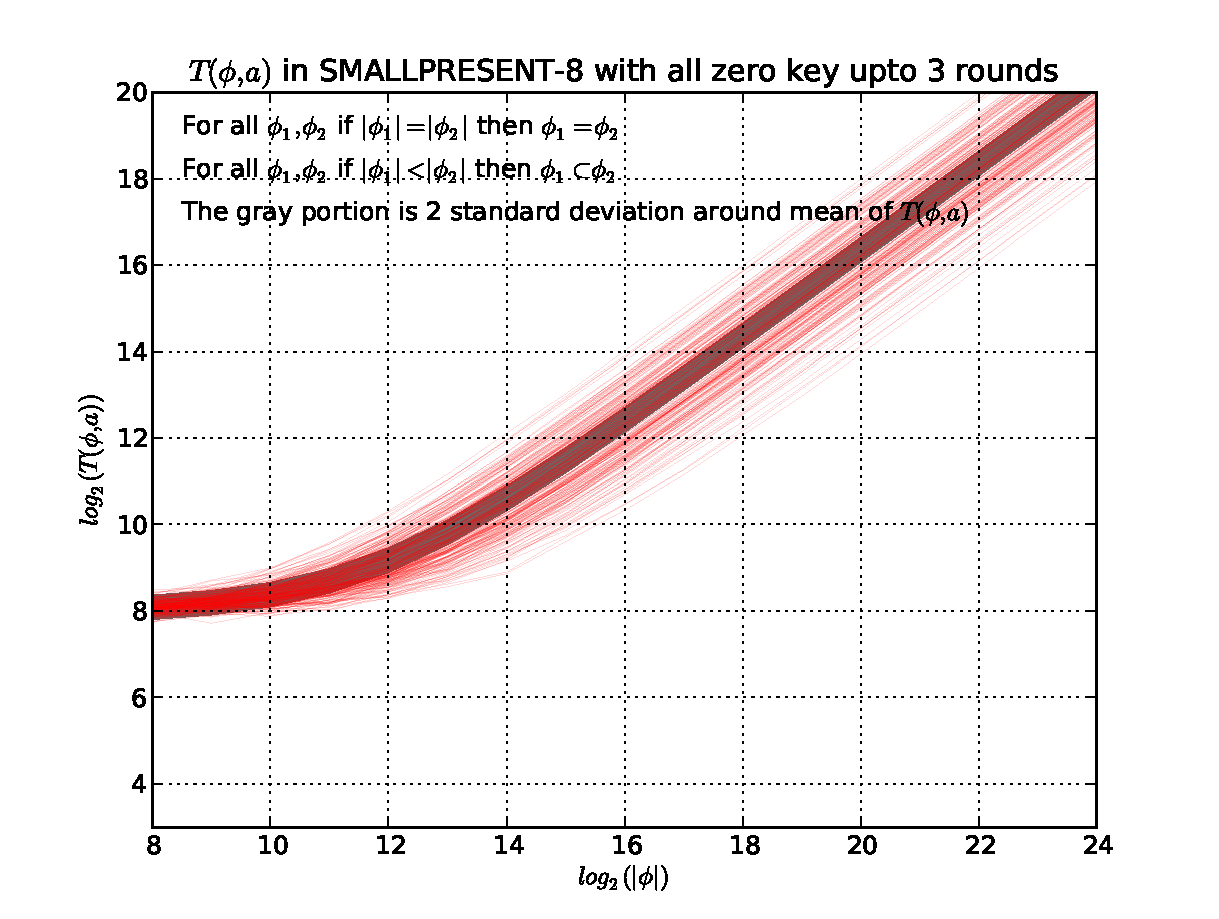
\includegraphics[width=\textwidth , height = 8cm]{T_a_phi_variable_a_varible_phi_variable_size_03rounds}
    \caption{$T(\phi,a)$ with $3$ rounds}
    \label{fig:T_a_phi_variable_a_varible_phi_variable_size_03rounds}
\end{figure}

\begin{figure}[h!]
    \centering
    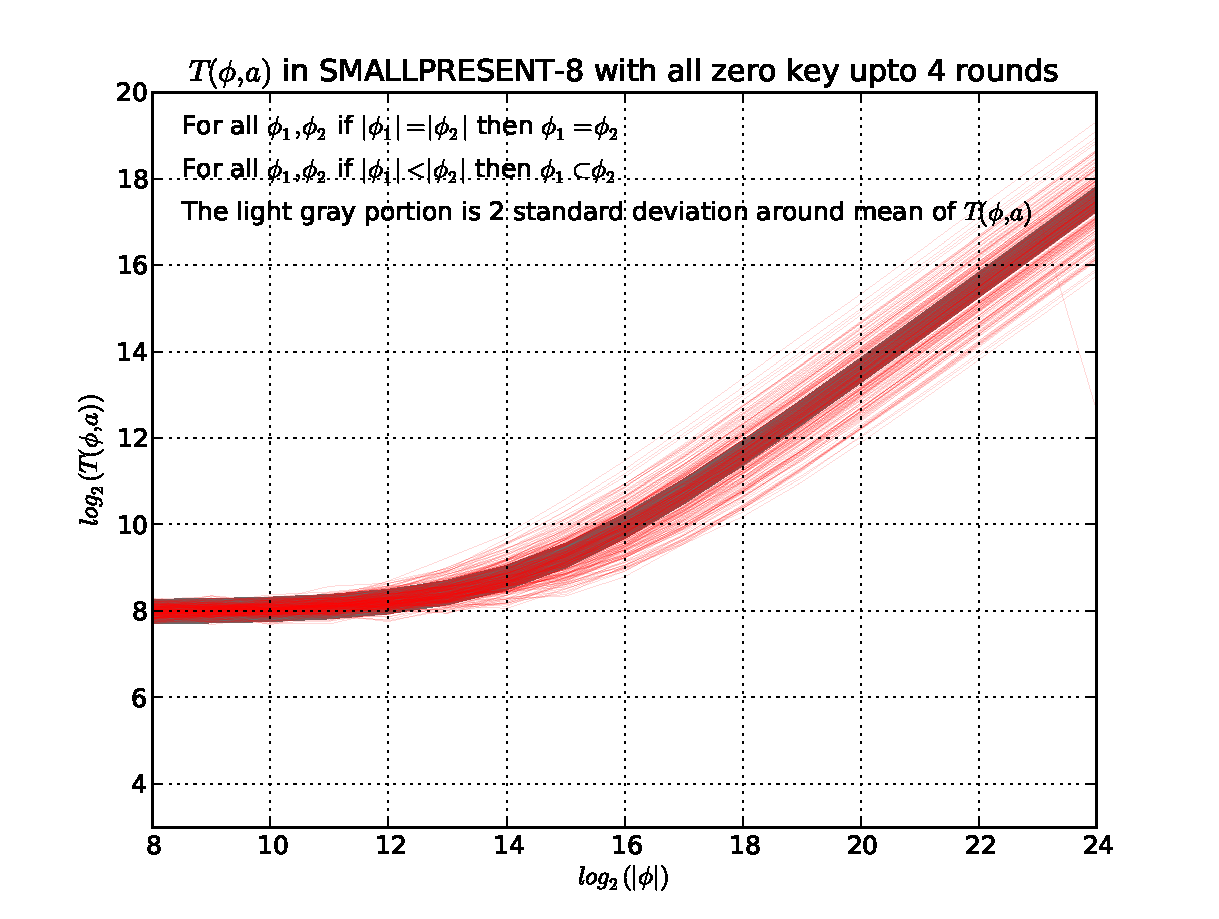
\includegraphics[width=\textwidth , height = 8cm]{T_a_phi_variable_a_varible_phi_variable_size_04rounds}
    \caption{$T(\phi,a)$ with $4$ rounds}
    \label{fig:T_a_phi_variable_a_varible_phi_variable_size_04rounds}
\end{figure}

\begin{figure}[h!]
    \centering
    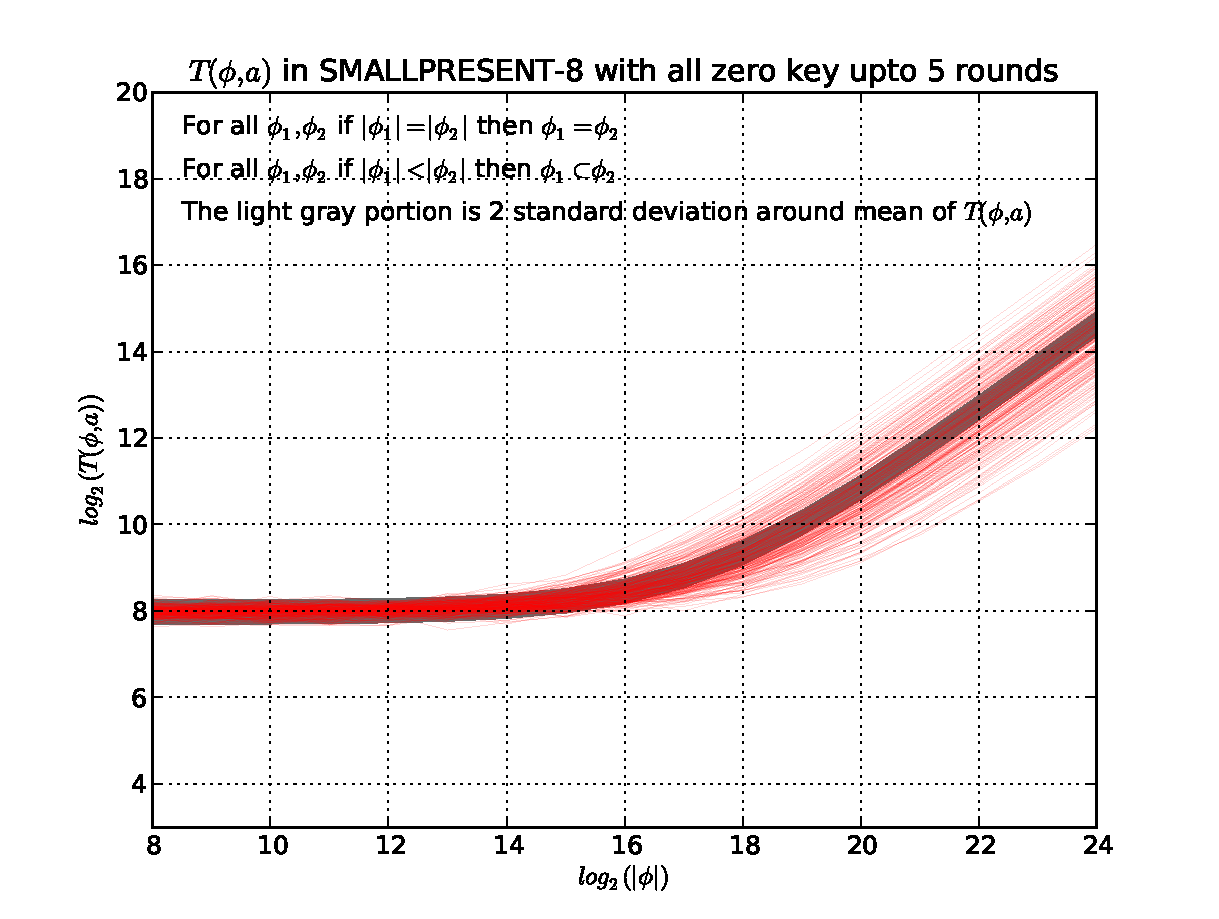
\includegraphics[width=\textwidth , height = 8cm]{T_a_phi_variable_a_varible_phi_variable_size_05rounds}
    \caption{$T(\phi,a)$ with $5$ rounds}
    \label{fig:T_a_phi_variable_a_varible_phi_variable_size_05rounds}
\end{figure}

\begin{figure}[h!]
    \centering
    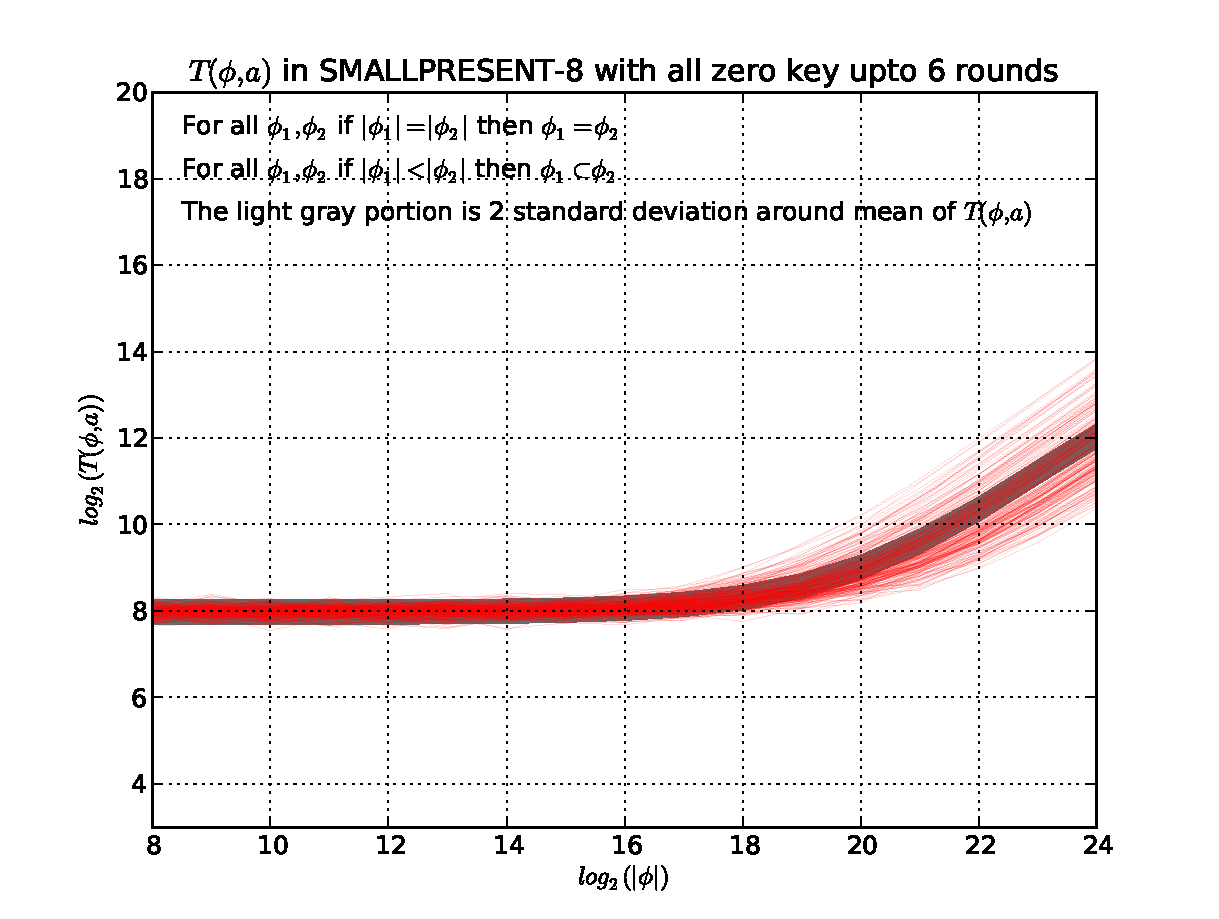
\includegraphics[width=\textwidth , height = 8cm]{T_a_phi_variable_a_varible_phi_variable_size_06rounds}
    \caption{$T(\phi,a)$ with $6$ rounds}
    \label{fig:T_a_phi_variable_a_varible_phi_variable_size_06rounds}
\end{figure}

\begin{figure}[h!]
    \centering
    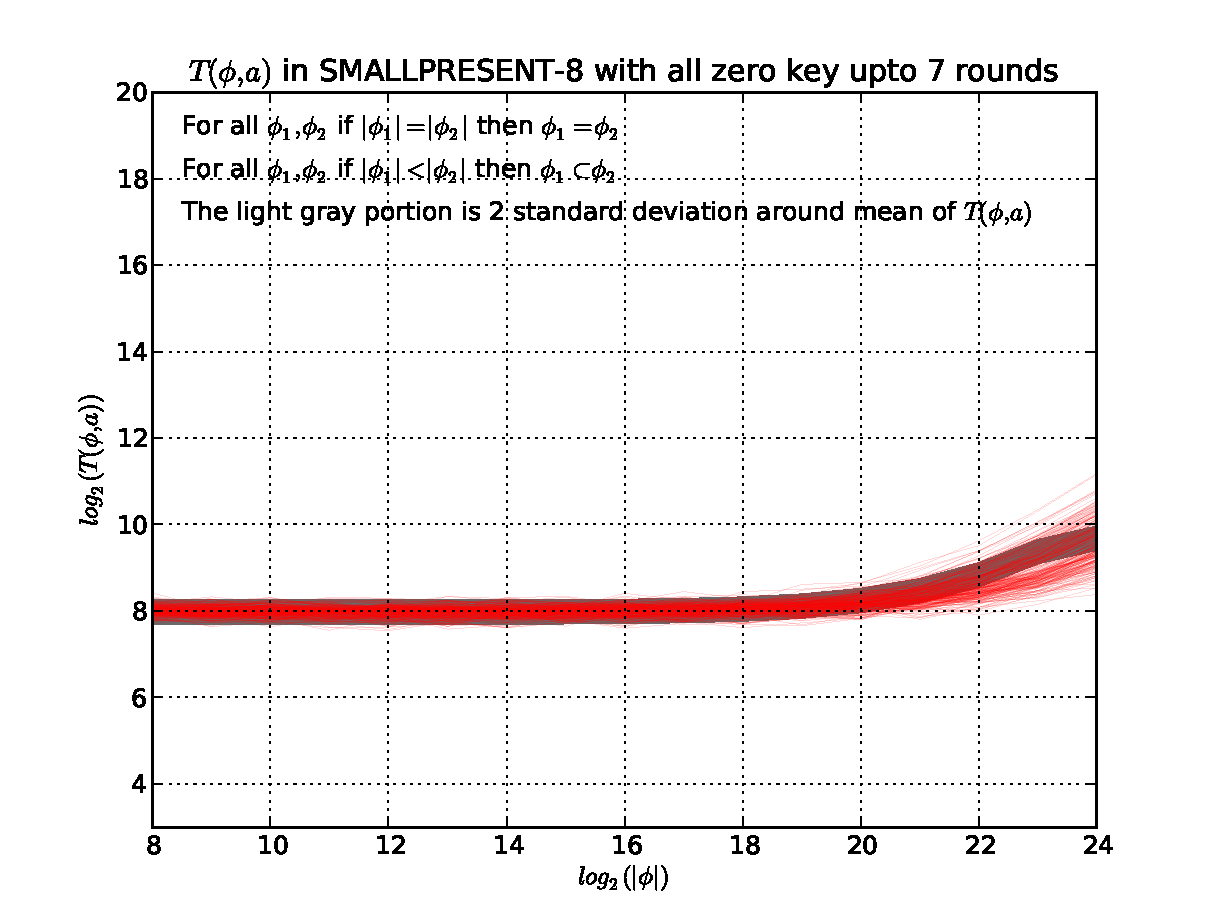
\includegraphics[width=\textwidth , height = 8cm]{T_a_phi_variable_a_varible_phi_variable_size_07rounds}
    \caption{$T(\phi,a)$ with $7$ rounds}
    \label{fig:T_a_phi_variable_a_varible_phi_variable_size_07rounds}
\end{figure}

\begin{figure}[h!]
    \centering
    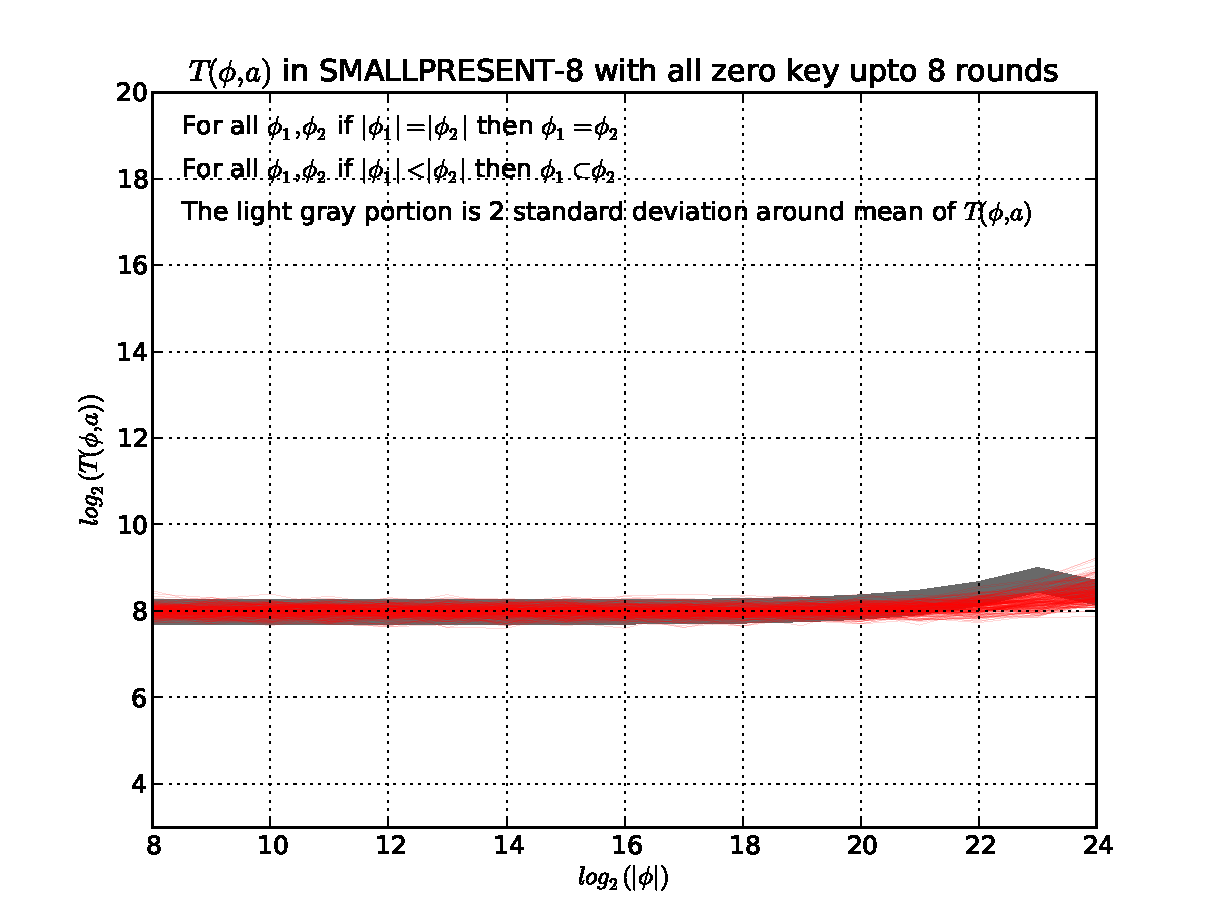
\includegraphics[width=\textwidth , height = 8cm]{T_a_phi_variable_a_varible_phi_variable_size_08rounds}
    \caption{$T(\phi,a)$ with $8$ rounds}
    \label{fig:T_a_phi_variable_a_varible_phi_variable_size_08rounds}
\end{figure}

\begin{figure}[h!]
    \centering
    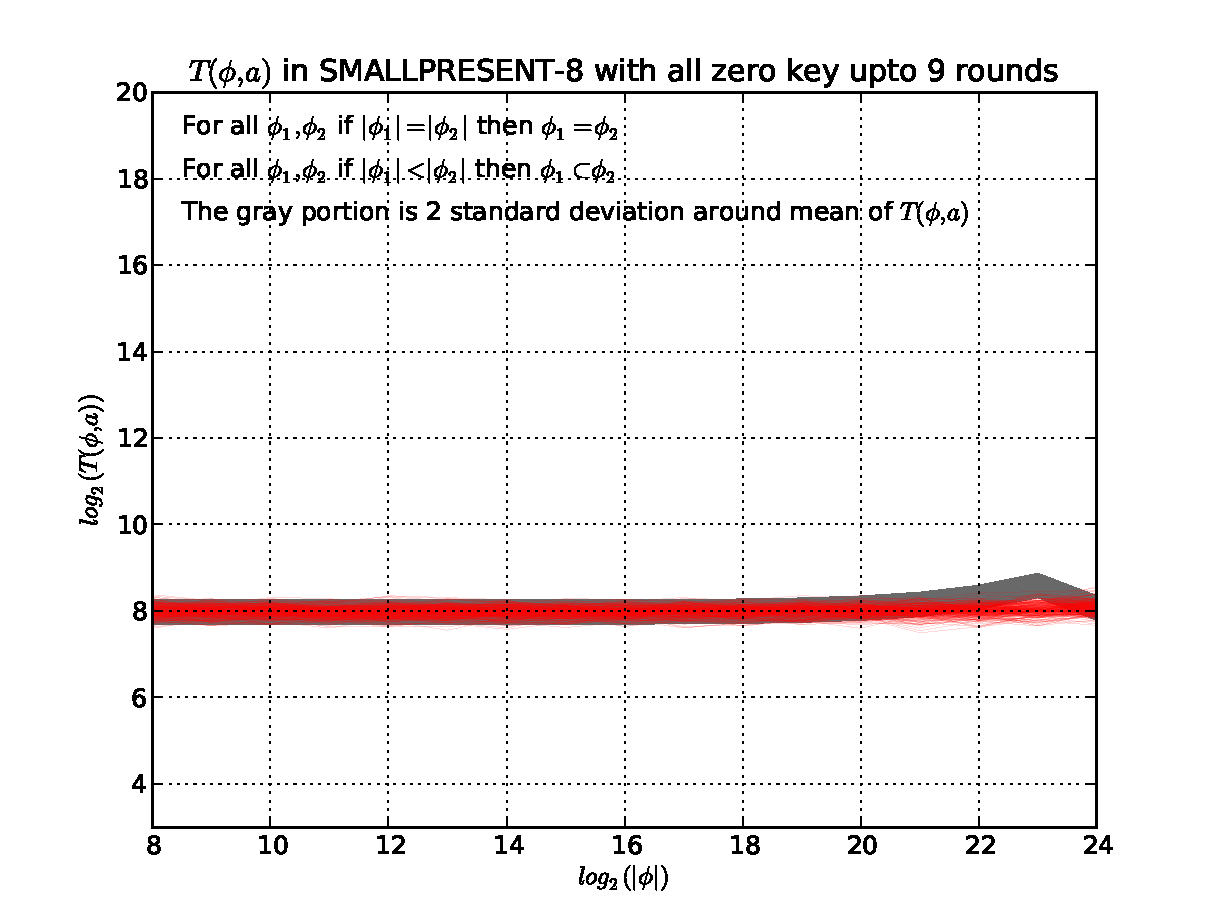
\includegraphics[width=\textwidth , height = 8cm]{T_a_phi_variable_a_varible_phi_variable_size_09rounds}
    \caption{$T(\phi,a)$ with $9$ rounds}
    \label{fig:T_a_phi_variable_a_varible_phi_variable_size_09rounds}
\end{figure}

\begin{figure}[h!]
    \centering
    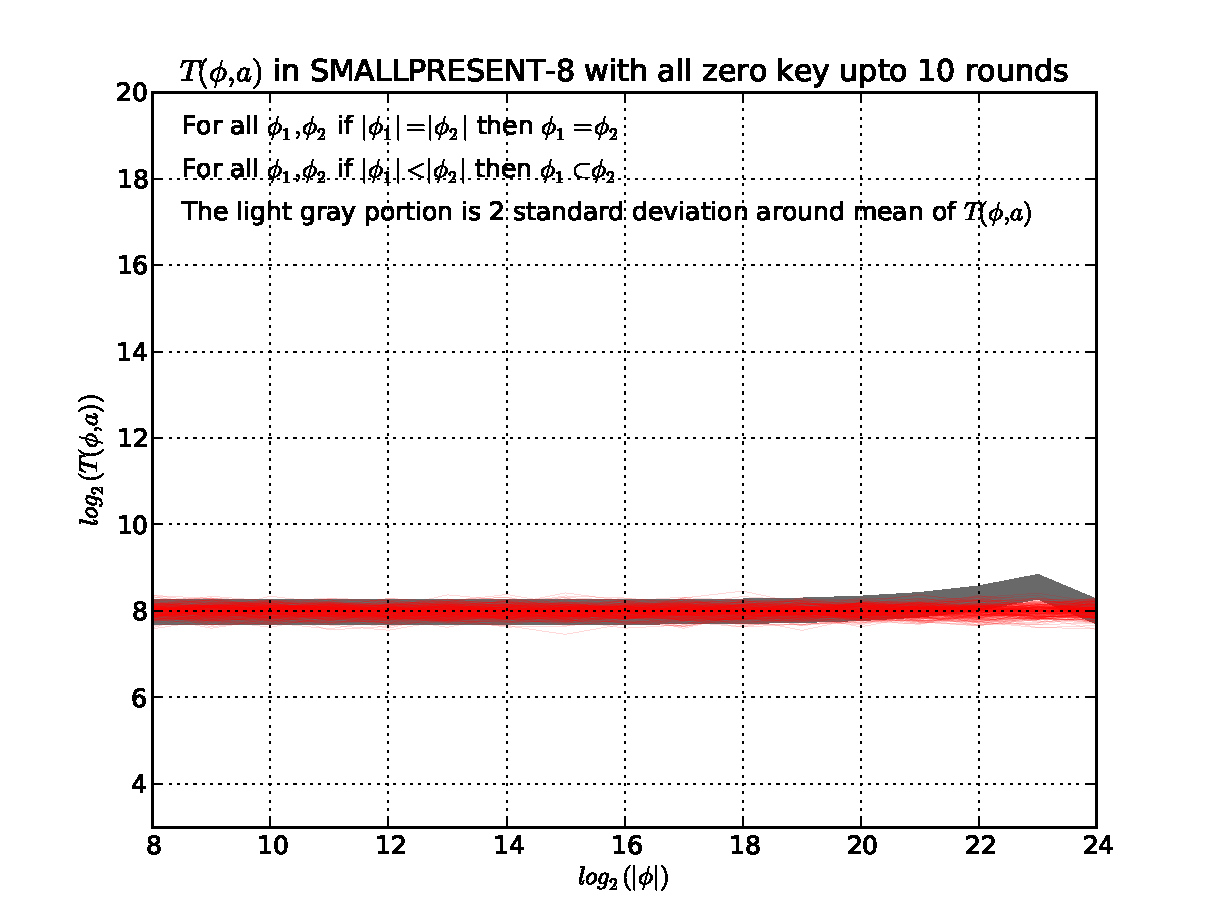
\includegraphics[width=\textwidth , height = 8cm]{T_a_phi_variable_a_varible_phi_variable_size_10rounds}
    \caption{$T(\phi,a)$ with $10$ rounds}
    \label{fig:T_a_phi_variable_a_varible_phi_variable_size_10rounds}
\end{figure}

\begin{figure}[h!]
    \centering
    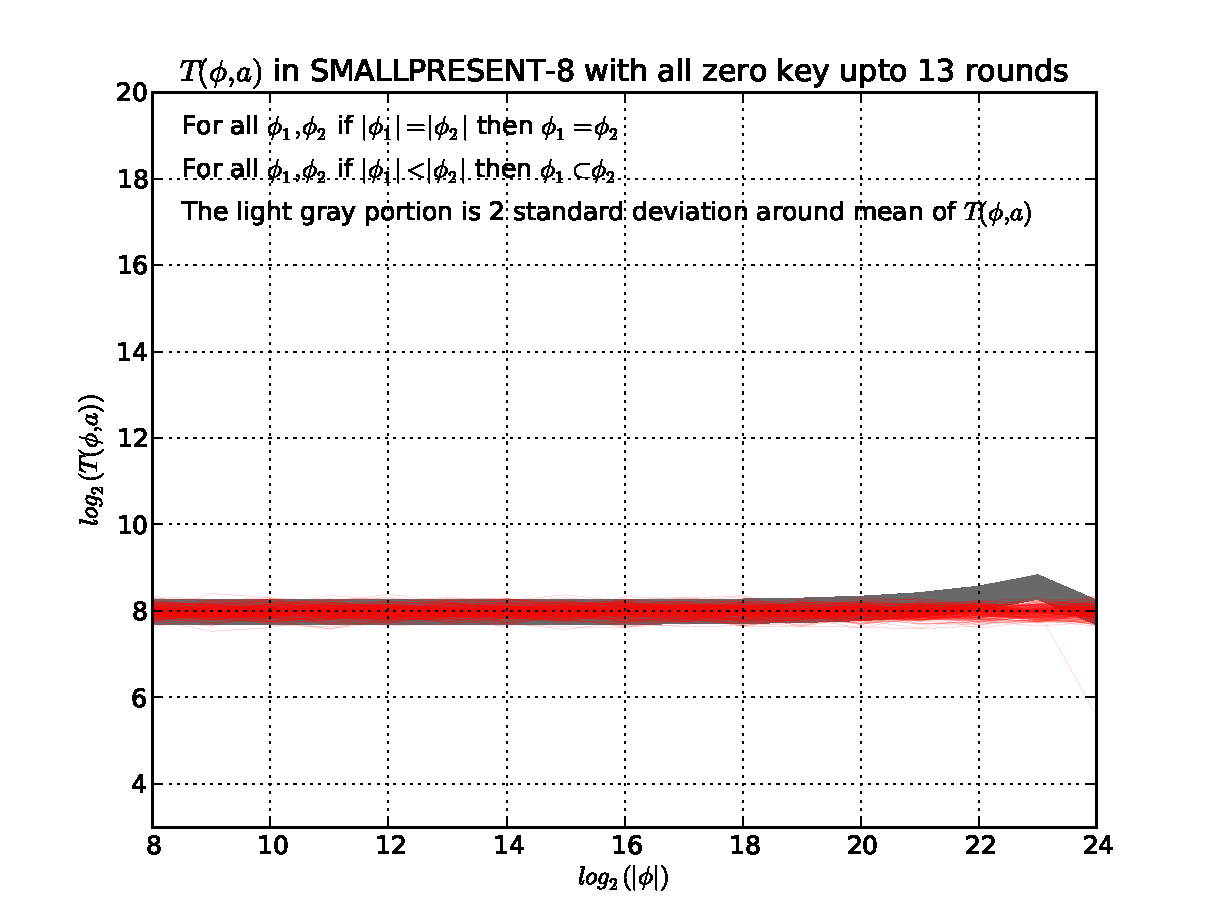
\includegraphics[width=\textwidth , height = 8cm]{T_a_phi_variable_a_varible_phi_variable_size_13rounds}
    \caption{$T(\phi,a)$ with $13$ rounds}
    \label{fig:T_a_phi_variable_a_varible_phi_variable_size_13rounds}
\end{figure}

\end{document}